\documentclass[11pt,letterpaper]{article}

\usepackage[utf8]{inputenc}
\usepackage[spanish,es-nodecimaldot]{babel}

\usepackage[top=1in, bottom=1in, left=1in, right=1in]{geometry}

\usepackage{xcolor}
\usepackage{color}
\usepackage{graphicx}
\usepackage{minted}

\usemintedstyle{pastie}
\definecolor{MBckg}{HTML}{272822}

\begin{document}

\begin{titlepage}
    \centering

    {\scshape\LARGE Universidad Nacional Autónoma de México \par}

    \vspace{1cm}
    {\scshape\Large Facultad de Ciencias\par}
    \vspace{1.5cm}

    \begin{center}
        
\includegraphics[scale=.1]{../../assets/img/logo.png}
    \end{center}

    \vspace{.8 cm}

    {\LARGE Práctica 02: \par}
    {\huge\bfseries Tipos primitivos y bits \par}

    \vspace{0.5cm}
    {\large\itshape Pablo A. Trinidad Paz\par}

    \vfill

    Trabajo presentado como parte del curso de \textbf{Introducción a Ciencias de la Computación}
    impartido por la profesora \textbf{Verónica Esther Arriola Ríos}. \par
    \vspace{0.1cm}
    {\large 27 de agosto de 2018\par}
\end{titlepage}

{\LARGE Actividades \par}

\textbf{Actividad 2.1} Revisa la documentación de las clases \texttt{Byte},
\texttt{Short}, \texttt{Integer} y \texttt{Long} de \texttt{Java} y revisa
los atributos de clase que permiten acceder a esta información
\textbf{a)} ¿Cuáles encuentras relevantes? \\

Intenta sumarle uno a \texttt{max}, imprime el resultado en base 10 y su
representación en binario. \textbf{b)} Explica qué pasó.

\begin{enumerate}
    \item[a)] Todos los considero relevantes excepto por \texttt{TYPE} y \texttt{BYTES}
    porque creo que son muy redundantes. Respecto a \texttt{BYTES}, ya contamos con
    \texttt{SIZE} el cual menciona el número de bits y respecto a \texttt{TYPE} pues
    también siento muy redundante preguntar de qué clase viene el número si cuando
    lo inicializamos ya lo decimos explicitamente, por ejemplo:
        \begin{minted}[fontsize=\footnotesize,baselinestretch=1,gobble=8]{java}
            double n = Double.MAX_VALUE;
            n.TYPE; // <--- ¿?
        \end{minted}

    \item[b)] El valor de \texttt{max} es $2147483647_{10}$ en base 10 el cuál es equivalente
    a 31 $1s$ precedidos por un $0$ en base 2 ($01111111111111111111111111111111_2$)
    donde el $0$ indica que se trata de un entero positivo y al mismo tiempo se hace uso
    de los 32 bits. Al momento de sumar 1 al valor de \texttt{max}, la representación
    resultante en base 2 se vuelve $10000000000000000000000000000000_2$ la cuál es
    interpretada dentro de Java como un entero negativo debido a que el primer dígito
    indica el signo, y a su vez, el valor de \texttt{max} es equivalente a $-2147483648_{10}$
    en base 10.
\end{enumerate}

\textbf{Actividad 2.2} Utiliza la clase \texttt{ImpresoraBinario} para visualizar
la representación interna de estos\footnote{Referente a los valores descritos
dentro de la descripción de la práctica.} valores especiales.

    \begin{center}
        \begin{tabular}{ l | c c }
        Valor & Base 2 \\
        \hline
        \texttt{NaN} & $111111111111000000000000000000000000000000000000000000000000000_2$ \\
        \texttt{NEGATIVE\_INFINITY} & $1111111111110000000000000000000000000000000000000000000000000000_2$ \\
        \texttt{POSITIVE\_INFINITY} & $111111111110000000000000000000000000000000000000000000000000000_2$ \\
        \texttt{$0.0$} & $0_2$ \\
        \texttt{$-0.0$} & $1000000000000000000000000000000000000000000000000000000000000000_2$
        \end{tabular}
    \end{center}

\textbf{Actividad 2.3} Imprime como se ve esto en binario ¿Cuánto vale \texttt{permisos}
en base 10? (Sólo mándalo a imprimir \texttt{Java} tabaja por defecto en base 10) \\

    El código:

    \begin{minted}[fontsize=\footnotesize,baselinestretch=1,gobble=8]{java}
        ImpresoraBinario printer = new ImpresoraBinario();
        int permisos = Integer.parseInt("0754", 8);
        printer.imprime(permisos);
        System.out.println(permisos);
    \end{minted}

    Genera la salida:
    \begin{verbatim}
111101100
492
    \end{verbatim}

\textbf{Actividad 2.4} Realiza pruebas con los operadores de corrimiento $<<$, $>>$ y $>>>$.
Recorre los números del inciso anterior por uno y tres bits. \\

    El código:

    \begin{minted}[fontsize=\footnotesize,baselinestretch=1,gobble=8]{java}
        System.out.println("\n\n====== Actividad 2.4 ======");

        ImpresoraBinario printer = new ImpresoraBinario();
        int permissions_b10 = 0754;

        System.out.print("Original value: ");
        printer.imprime(permissions_b10);

        System.out.print("\n<< 1: ");
        printer.imprime(permissions_b10 << 1);
        System.out.print("<< 3: ");
        printer.imprime(permissions_b10 << 3);

        System.out.print("\n>> 1: ");
        printer.imprime(permissions_b10 >> 1);
        System.out.print(">> 3: ");
        printer.imprime(permissions_b10 >> 3);

        System.out.print("\n>>> 1: ");
        printer.imprime(permissions_b10 >>> 1);
        System.out.print(">>> 3: ");
        printer.imprime(permissions_b10 >>> 3);
    \end{minted}

    Genera la salida:
    \begin{verbatim}
====== Actividad 2.4 ======
Original value: 111101100

<< 1: 1111011000
<< 3: 111101100000

>> 1: 11110110
>> 3: 111101

>>> 1: 11110110
>>> 3: 111101
    \end{verbatim}

\textbf{Actividad 2.5} Ahora toma los permisos de la sección anterior: ¿Qué
operaciones necesitas hacer para que todos los usuarios tengan permiso de
escritura? Verifica tu respuesta imprimiendo las representaciones binarias. \\

    Podemos hacer uso de la operación \textbf{or} y el valor 1 en la posición
    de los permisos de escritura (tercer caracter de cada grupo de usuarios)
    y usar el valor 0 para las demás posiciones y para no alterar los valores
    de otros permisos. Dicho de otra manera, le aplicamos la función \textbf{or}
    a cualquier permiso existente usando el valor \textbf{$010010010_2$} ($222_8$). \\

    \clearpage
    Verificación:

    \begin{minted}[fontsize=\footnotesize,baselinestretch=1,gobble=8]{java}
        System.out.println("\n\n====== Actividad 2.5 ======");

        ImpresoraBinario printer = new ImpresoraBinario();
        int original_permission = 0754;
        int write_permissions = 0222;

        System.out.print("Original value: ");
        printer.imprime(permission);

        System.out.print("Write permissions: ");
        printer.imprime(write_permissions);

        System.out.print("New permission (original OR write): ");
        printer.imprime(permission | write_permissions);
    \end{minted}

    Genera la salida:
    \begin{verbatim}
====== Actividad 2.5 ======
Original value: 111101100
Write permissions: 10010010
New permission (original OR write): 111111110
    \end{verbatim}

{\LARGE Ejercicios \par}

\textbf{Ejercicio 1} Almacena el valor \textbf{456} en diferentes tipos primitivos,
muestra su representación binaria y explica las diferencias que observas. \\

    \begin{center}
        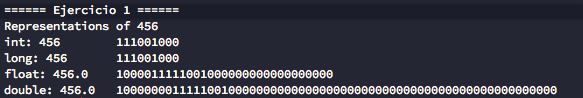
\includegraphics[scale=.7]{assets/img/e-1.png}
    \end{center}

    La diferencia más obvia es la cantidad de bits que utiliza cada tipo de dato aunque
    rápidamente podemos encontrar la similitud de que el valor \textbf{111001000} siempre
    forma parte de la representación binaria. También se puede distinguir que el tamaño
    de la matiza de un double aumenta.\\

\textbf{Ejercicio 2} Repite los mismos pasos del ejercicio anterior, pero ahora con \textbf{-456}.

    \begin{center}
        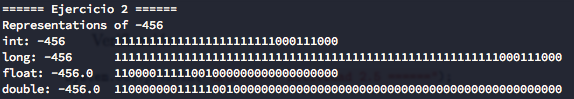
\includegraphics[scale=.7]{assets/img/e-2.png}
    \end{center}

    En esta ocasión los primeros bits de \texttt{int} y \texttt{long} ya son usa dos y
    los flotantes cambian los primeros valores de la parte del exponent a 1.\\

\textbf{Ejercicio 3} Repite los mismos pasos pero con -456.601. Ojo, en este caso deberás
hacer un casting para guardar el número en los tipos correspondientes a enteros y perderás
la parte fraccionaria. ¿Qué número queda almacenado?

    \begin{center}
        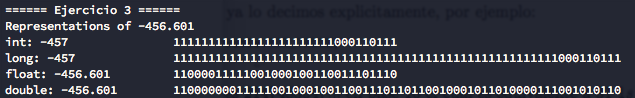
\includegraphics[scale=.7]{assets/img/e-3.png}
    \end{center}

    El número almacenado es 457 debido a que hace un redondeo del valor decimal.\\

\textbf{Ejercicio 4} Finalmente, crea un \texttt{int} llamada \texttt{mascara} cuyos
últimos dígitos sean $1s$. Ahora utiliza el operador de corrimiento necesario para
colocarlos en las posiciones 4 a la 7 (contando de derecha a izquierda). ¿Qué número
obtienes?

    \begin{center}
        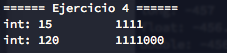
\includegraphics[scale=.7]{assets/img/e-4.png}
    \end{center}

\textbf{Ejercicio 5} Dado un \texttt{int num = 1408}, realiza la operación \texttt{num \& mascara}.
Imprime los bits resultantes y el valor numérico del resultado. Repite el ejerciio con \texttt{|}
y \texttt{$\sim$}.

    \begin{center}
        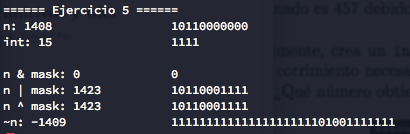
\includegraphics[scale=.8]{assets/img/e-5.png}
    \end{center}

\end{document}
